\documentclass{beamer}

\usetheme{AUTheme}
\usefonttheme[onlymath]{serif}

\usepackage{amsmath, latexsym, color, graphicx, amssymb, here}
\usepackage{epsf, epsfig, pifont,tikz}
\usepackage{graphics, calrsfs}
\usepackage{tangocolors}
\usepackage{times}
\usepackage{fancybox,calc}
\usepackage{hyperref}
\usepackage{pgfplots}

\newcommand{\parD}[2]{\frac{\partial #1}{\partial #2}}
\newcommand{\parDD}[2]{\frac{\partial^2 #1}{\partial #2 ^2}}
\newcommand{\laplacian}{\Delta}
\renewcommand{\div}{\nabla\cdot}
\newcommand{\grad}{\nabla}
\newcommand{\divp}{\nabla^\prime\cdot}
\newcommand{\gradp}{\nabla^\prime}
\newcommand{\curl}{\nabla\times}
\newcommand{\cross}{\times}
\renewcommand{\dot}{\cdot}
% define some colors
\definecolor{cBlue}{rgb}{.255,.41,.884} % RoyalBlue of svgnames
\definecolor{cRed}{rgb}{1, 0, 0} % Red of svgnames



%\usecolortheme[named=blue]{structure}

\title{Introducing Document Preparation with  \LaTeX }
\author{{Stan Reeves}}
\institute{Department of Electrical and Computer Engineering}
\date{\today}

\begin{document}


\frame{\titlepage}
%\slideCaption{\LaTeX}

%------------------------------------------------------------Slide 1
\section{Introduction}
\frame
{
\frametitle{\TeX\ }
\begin{itemize}

    \item Preparation of a document involves
    \begin{itemize}
        \item Entering text
        \item \textcolor[rgb]{0.00,0.00,1.00}{Formatting text}
        \item Display on a screen
        \item Printing
    \end{itemize}
\pause
    \item \TeX\ ($\tau\epsilon\chi$) is a typesetting system.
    \begin{itemize}
        \item METAFONT -- Font description language
        \begin{itemize}
            \item A point on a glyph is found as the intersection of a line segment and a B\'{e}zier cubic curve
        \end{itemize}
        \item Computer modern typeface.
        \begin{itemize}
            \item 62 parameters control the widths and heights of elements
        \end{itemize}
    \end{itemize}
\end{itemize}
\setbeamercolor{uppercol}{fg=white,bg=ta3orange}%
\setbeamercolor{lowercol}{fg=black,bg=taorange}%
\begin{beamerboxesrounded}[upper=uppercol,lower=lowercol,shadow=true]
{Author of \TeX\ }
Donald Knuth (1978), computer science professor at Stanford
\end{beamerboxesrounded}

}


\frame
{
\frametitle{\TeX\ and \LaTeX}
\begin{itemize}
\item<1-> Math spacing carefully derived based on typesets in:
\begin{itemize}
\item \emph{Acta Mathematica}
\item \emph{Indagationes Mathematicae}
\item Addison-Wesley's books
\end{itemize}
\item<2-> Line breaks
\begin{itemize}
\pause
\item A {\em total-fit} line-breaking algorithm
\item Assigns {\em badness}. Minimizes SS of badness
\end{itemize}
\pause
\item<3-> Hyphenation algorithm
\begin{itemize}
\item Removes prefixes and suffixes
\item Will attempt to put a break between consonants in a pattern of the form
vowel-consonant-consonant-vowel.
\end{itemize}
\end{itemize}
\pause

\setbeamercolor{uppercol}{fg=white,bg=ta3orange}%
\setbeamercolor{lowercol}{fg=black,bg=taorange}%
\begin{beamerboxesrounded}[upper=uppercol,lower=lowercol,shadow=true]
{\LaTeX\ is a set of macros for \TeX\ }
Written by Leslie Lamport (1984), current release \LaTeX$2_\varepsilon$
\end{beamerboxesrounded}

}


\frame
{
\frametitle{Pronunciation of \LaTeX}
\begin{itemize}
\item no single agreed-upon pronunciation
\item \TeX\ derives from the Greek $\tau\epsilon\chi\nu\eta$, which means ``art, skill, craft''
\item origin of the name suggests that ``X'' be pronounced like the ``ch'' in ``technical''
\item Options:
\begin{itemize}
\item LAYtek
\item LAHtek
\item LahTEK
\end{itemize}
\end{itemize}

}


\frame
{
\frametitle{Why \LaTeX?}
\begin{itemize}
\item It is a natural choice if you want to create beautiful output
\item A structured system of typesetting. Spend time and effort on content not on layout
\item Works across platforms
\item Handles math well
\item Table of contents, list of figures, bibliography etc.
\item Cross-referencing features
\item Stable processing engine
\item Highly extensible
\item Input is plain text
\item Output can be anything
\item Complete document preparation. Articles, presentations, posters, HTML.
\pause
\item {\textcolor[rgb]{1.00,0.00,0.00}{FREE \& open source}}
\end{itemize}
}




%------------------------------------------------------------Slide 2

\frame
{
\frametitle{\LaTeX \ vs. MS Word}
\begin{center}
\begin{tabular}{lcc}
  % after \\ : \hline or \cline{col1-col2} \cline{col3-col4} ...
  {}            &        \LaTeX           & MS Word   \\ \hline \hline
  WYSIWYG       &  $\times$          &  $\textcolor[rgb]{0.00,0.00,1.00}{\checkmark}$ \\
  Platform independent   &$ \textcolor[rgb]{0.00,0.00,1.00}{\checkmark}$    &  $\times$ \\
  Math                   & $\textcolor[rgb]{0.00,0.00,1.00}{\checkmark}$ & $ \textcolor[rgb]{1.00,0.00,1.00}{\checkmark}$  \\
  Citations \& references   & $\textcolor[rgb]{0.00,0.00,1.00}{\checkmark}$    &$  \times $\\
  Automated TOC, LoF   &     $\textcolor[rgb]{0.00,0.00,1.00}{\checkmark} $ & $ \times $\\
  Cross-references    & $\textcolor[rgb]{0.00,0.00,1.00}{\checkmark}$ & $\times  $     \\
  Style changes       & $\textcolor[rgb]{0.00,0.00,1.00}{\checkmark}$ & $\textcolor[rgb]{1.00,0.00,1.00}{\checkmark}$        \\
  Multimedia                 & $\textcolor[rgb]{1.00,0.00,1.00}{\checkmark}$ & $ $\textcolor[rgb]{0.00,0.00,1.00}{\checkmark}$    $ \\
  Free                 & $\textcolor[rgb]{0.00,0.00,1.00}{\checkmark}$ & $ \times    $ \\

\end{tabular}
\end{center}
}



\frame
{
\frametitle{Why \LaTeX?}
\vspace{1cm}
\uncover<2->{\textcolor{ta3chameleon}{\LaTeX\ }}

\uncover<1->{
\begin{align*}
I_{mn}(\lambda)&=I_0(\lambda) T_m^2(\lambda)
\sum_{p=-\infty}^{\infty} \int_{r_m}^{r_m+w_m} dx\, \int_{rn+pT}^{r_n+w_m+pT} \mathrm{PSF}(x-x')dx'
\end{align*}
}

\uncover<2->{\textcolor{tascarletred}{MS Word Equation Editor}}
\uncover<1->{
\begin{figure}[!h]
\centering
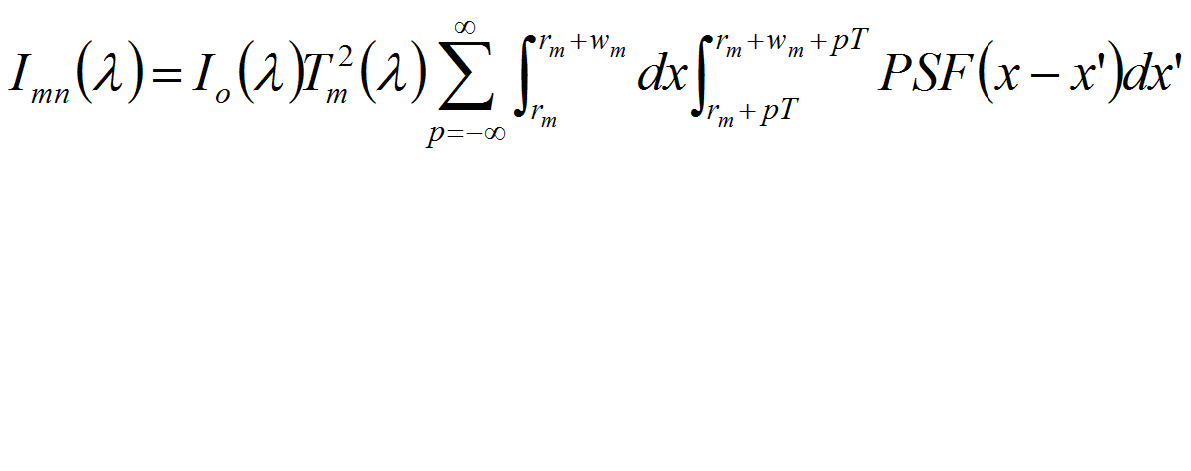
\includegraphics[width = 9cm]{wordEquation.png}
\end{figure}
}

}


%------------------------------------------------------------Slide


\frame {\frametitle{Why \LaTeX?}
\vspace{-10pt}
\begin{figure}[!h]
\centering
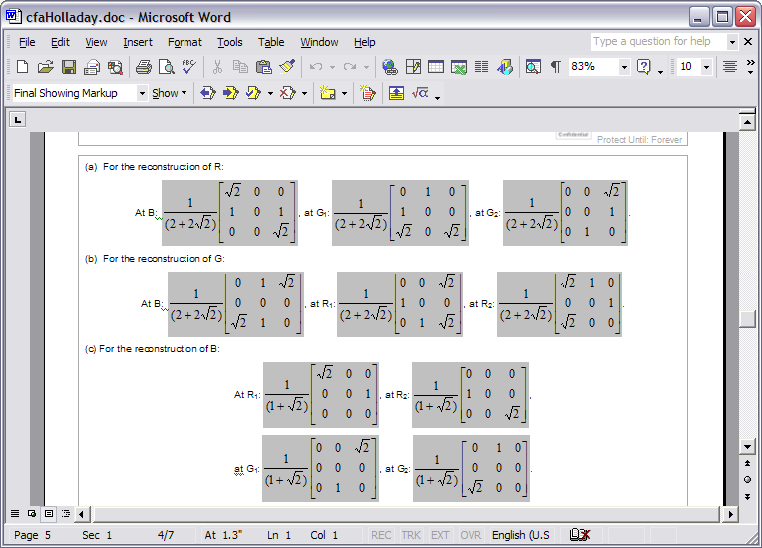
\includegraphics[width = 9cm]{wordEquations.png}
\end{figure}
}


%------------------------------------------------------------Slide

\frame { \frametitle{Installation}

\setbeamercolor{uppercol}{fg=white,bg=ta3orange}%
\setbeamercolor{lowercol}{fg=black,bg=taorange}%
\begin{beamerboxesrounded}[upper=uppercol,lower=lowercol,shadow=true]{Packages}
\begin{center}
\begin{tabular}{lcc}
  {}            & Back-end          & Front-end  \\ \hline \hline
  Windows       & Mik\TeX\ ,  \TeX Live & WinEdt, \TeX nicCenter   \\
  Mac       &    CMac\TeX, Oz\TeX  &  \TeX Shop i\TeX Mac \\
  Linux         & te\TeX , \TeX\ Live     & Kile
\end{tabular}
\end{center}
\end{beamerboxesrounded}

\vspace{0.5cm}
CoE Windows labs have:
\begin{itemize}
\item  Mik\TeX\
\item  \TeX nicCenter
\end{itemize}
}



%%----------------------------------------------
\frame
{
\frametitle{\LaTeX \ for the PC}
To install \LaTeX \ on your PC you need:
\begin{itemize}
    \item \textcolor{cRed}{The back-end}: The base \TeX\ package
\begin{itemize}
\item Windows
\begin{itemize}
    \item (Mik\TeX). \ Available at \href{http://www.miktex.org}{\underline{\textcolor[rgb]{0.00,0.00,1.00}{the Mik\TeX}} homepage}
    \item \TeX Live
    \item Ghostscript, Ghostview, and GSview.
    \end{itemize}
\end{itemize}
    \item \textcolor{cRed}{The front-end}: A \LaTeX \ editor (WinEdt, \TeX nicCenter)
    \begin{itemize}
    \item WinEdt: evaluation version. \TeX nicCenter: free
    \item Available at \href{http://www.winedt.com}{\underline{\textcolor[rgb]{0.00,0.00,1.00}{the WinEdt}} homepage} \\
              or at \href{http://sourceforge.net/projects/texniccenter/}{\underline{\textcolor[rgb]{0.00,0.00,1.00}{Sourceforge.net}}}
    \end{itemize}
\end{itemize}
}



%------------------------------------------------------------Slide

\frame {\frametitle{The downside}
There are certain ``disadvantages''
\begin{itemize}
\item Somewhat steep learning curve
\item Not interactive. Have to use pre-viewer before finalizing document
\item Difficult to create your own document type
\end{itemize}

}



%------------------------------------------------------------Slide


\frame {\frametitle{\LaTeX \ workflow}
\vspace{-10pt}
\begin{figure}[!h]
\centering
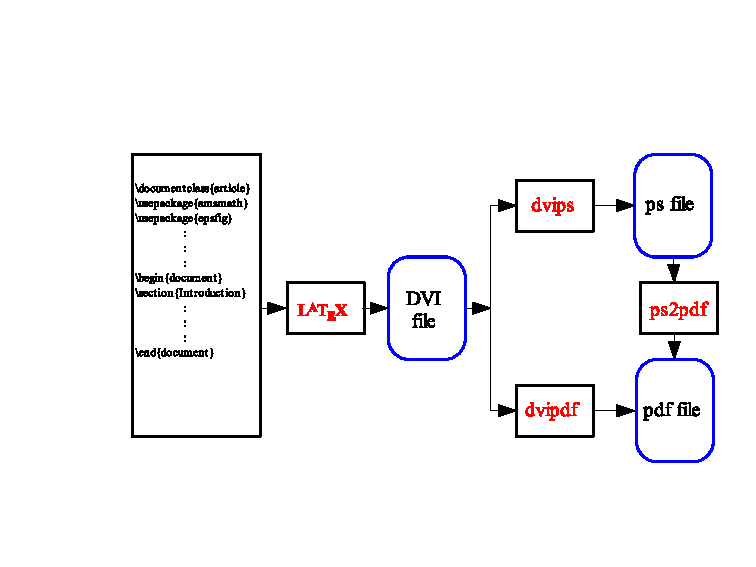
\includegraphics[width = 10cm]{latex_sys.pdf}
\end{figure}
\texttt{pdflatex} is an alternative workflow that goes straight from the *.tex file to a PDF file.
}




%------------------------------------------------------------Slide

\section{\LaTeX\ }

\begin{frame}[fragile]

\frametitle{Getting started}
{\fontsize{6}{8}\selectfont
\begin{verbatim}
\documentclass{article}

\begin{document}

\section{Introduction}

The conditional probability of an event $A$ assuming another
event $M$, denoted by $P(A\,|M)$, is by definition the ratio

\begin{align}
P(A\,|M) &= \frac{P(AM)}{P(M)}
\end{align}

\subsection{Bayes's theorem}

Bayes's theorem for probability densities is given by:

\begin{align}
p(x|y) &= \frac{p(y|x)p(x)}{p(y)}
\end{align}

\end{document}
\end{verbatim}}
\end{frame}


\frame {\frametitle{Getting started}
\vspace{-10pt}
\begin{figure}[h!]
\centering
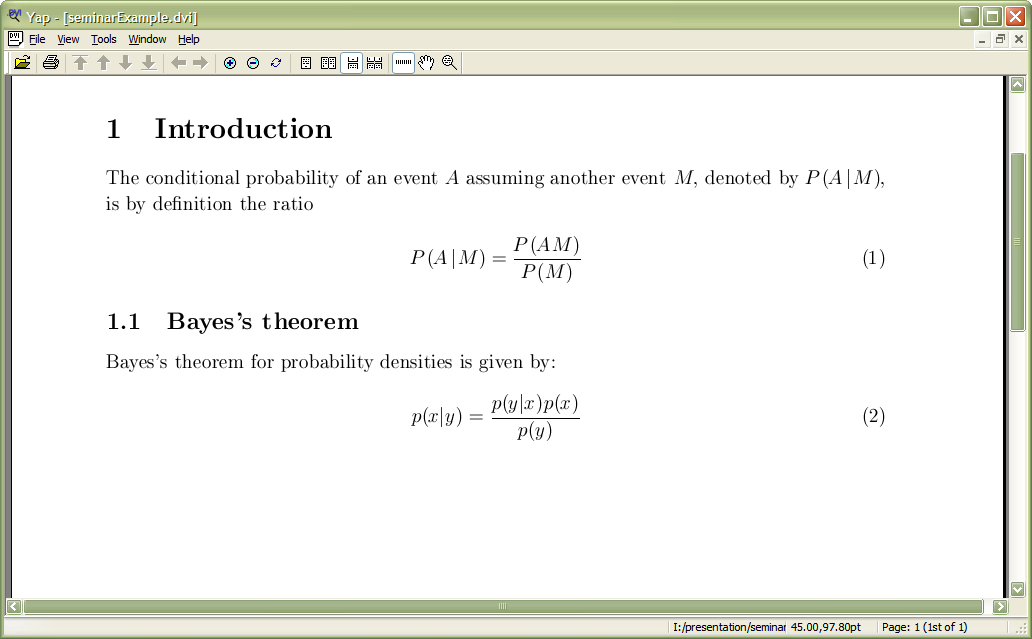
\includegraphics[width = 10cm]{seminarExample.png}
\end{figure}
}


%%------------------------------------------------------------------
\frame {\frametitle{LaTeX Documents}
\begin{itemize}
\item $\backslash$ is used to start \LaTeX \ commands
\item \% is used to start a comment
\item \&,  \$,  \#,  \_,  \^{},  \{ \} and \~{} are special characters
\item Words are separated by one or more spaces.
\item Paragraphs are separated by one or more blank lines.
\end{itemize}
}


%------------------------------------------------------------Slide
\begin{frame}[fragile]
\frametitle{Sectioning commands}

The sectional units in an article are produced by the following commands:
\begin{itemize}
\item \begin{verbatim} \chapter{title}\end{verbatim}
\item \begin{verbatim} \section{title} \end{verbatim}
\item \begin{verbatim} \subsection{title} \end{verbatim}
\item \begin{verbatim} \subsubsection{title}\end{verbatim}
\item \begin{verbatim} \paragraph{title} \end{verbatim}

\end{itemize}

\end{frame}


%------------------------------------------------------------Slide
\begin{frame} [fragile]

\frametitle{List Environments}
\vspace{-10pt}

{\fontsize{8}{10}\selectfont
\begin{verbatim}
\begin{itemize}
\item enumerate: Numbered lists
\item itemize: Bulletted lists
\end{itemize}
\end{verbatim}}

\begin{itemize}
\item enumerate: Numbered lists
\item itemize: Bulleted lists
\end{itemize}

{\fontsize{8}{10}\selectfont
\begin{verbatim}
\begin{enumerate}
\item enumerate: Numbered lists
\item itemize: Bulletted lists
\end{enumerate}
\end{verbatim}}

\begin{enumerate}
\item enumerate: Numbered lists
\item itemize: Bulletted lists
\end{enumerate}

\end{frame}


\begin{frame}[fragile]
\frametitle{Math}

\begin{itemize}
\item Inline math
{\fontsize{8}{10}\selectfont
\begin{verbatim}
Inline math appears within a line and must appear
enclosed in $ signs. $x^2 = 2
\Rightarrow x = \pm \sqrt{2}$.
\end{verbatim}}
Inline math appears within a line and must appear enclosed in \$ signs.
$x^2 = 2 \Rightarrow x = \pm \sqrt{2}$.

\item Equations
{\fontsize{8}{10}\selectfont
\begin{verbatim}
\begin{align}
\cal{F}(\omega) = \int _{-\infty}^{\infty}
f(t)e^{-j \omega t} dt
\end{align}
\end{verbatim}}
\setcounter{equation}{0}
\vspace{-10pt}
\begin{align}
{\cal{F}(\omega)} = \int_{-\infty}^{\infty}
f(t)\, e^{-j \omega t} dt
\end{align}
\end{itemize}

\end{frame}


%------------------------------------------------------------Slide
\begin{frame}[fragile]
\frametitle{More math}

{\fontsize{8}{10}\selectfont
\begin{verbatim}
The Fibonacci numbers form a sequence defined recursively by:
\begin{align}
F(n) &= \begin{cases}
            0, & \mbox{if} n=0;   \\
            1, & \mbox{if} n=1;   \\
            F(n-1) + F(n-2) \mbox{otherwise}.
        \end{cases}
\end{align}
\end{verbatim}}

\setcounter{equation}{2}
The Fibonacci numbers form a sequence defined recursively by:
\begin{align}
F(n) &= \begin{cases}
            0, & \mbox{if} \quad n=0;   \\
            1, & \mbox{if} \quad n=1;   \\
            F(n-1) + F(n-2) & \mbox{otherwise}.
        \end{cases}
\end{align}
\end{frame}





%%----------------------------------------

\begin{frame}[fragile]
\frametitle{Customizing}
{\fontsize{8}{10}\selectfont
\begin{verbatim}
\documentclass{article}
\newcommand{\parD}[2]{\frac{\partial #1}{\partial #2}}
\newcommand{\parDD}[2]{\frac{\partial^2 #1}{\partial^2 #2}}
\begin{document}

\begin{align*}
    \parD{}{x} \left( \parD{y}{x} \right) = \parDD{y}{x}
\end{align*}
\end{verbatim}
}

\begin{align*}
\parD{}{x} \left( \parD{y}{x} \right) = \parDD{y}{x}
\end{align*}

\end{frame}



%------------------------------------------------------------Slide

\begin{frame}[fragile]
\frametitle{Figures}

{\fontsize{6}{8}\selectfont

\begin{verbatim}
\documentclass{article}
\usepackage{graphicx}

\begin{figure}[!h]
\centering

\includegraphics[width=5cm]{ginn_logo.pdf}
\caption{CoE logo}
\end{figure}
\end{verbatim}}


\begin{minipage}{0.3\textwidth}
  \begin{center}

\includegraphics[width=0.75cm]{ginn_logo.pdf}
  \end{center}
\end{minipage}
%%% Titel
\begin{minipage}{0.35\textwidth}
  \begin{center}
    
\includegraphics[width=1.5cm]{ginn_logo.pdf}
  \end{center}
\end{minipage}
%%% GK-Logo
\begin{minipage}{0.3\textwidth}
  \begin{center}

\includegraphics[width=3cm]{ginn_logo.pdf}
\end{center}
\end{minipage}


\end{frame}

\frame
{
\frametitle{Video}

\vskip1.0in
\hskip0.3in

\hspace*{0.4in} \hbox{
\pdfannot width 220pt height 120pt depth 20pt{
%\pdfannot width 250pt height 188pt depth 40pt{
/Subtype /Movie
/T (Title)
/Movie <<
 /F (CYLIND03.AVI)
  /Poster true >>
/A << /ShowControls true /Mode /Open>>
}}

\vspace{0.2in}
\begin{center}Flow behind a cylinder - vorticity contours\end{center}

}
%/Rect [50 350 75 75]



\section{Editors}
%------------------------------------------------------------Slide

\frame {\frametitle{\TeX nicCenter}
\vspace{-10pt}
\begin{figure}[!h]
\centering
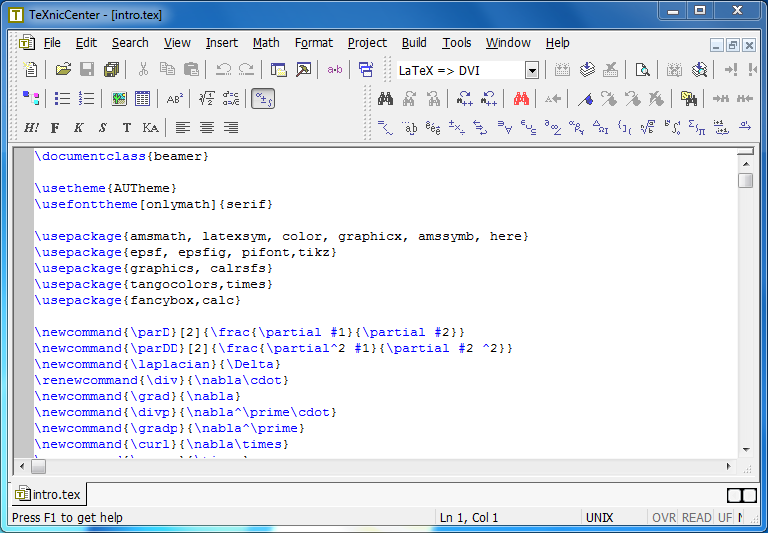
\includegraphics[width=10cm]{txc.png}
\end{figure}
\vspace{-10pt}

}


\section{Automation}
%%----------------------------------------------------------------------


\begin{frame}[fragile]
\frametitle{Cross-referencing}
\vspace{-8pt}
Can cross-reference figures, tables, equations, sections using:
{\fontsize{8}{10}\selectfont
\begin{verbatim}
\label{name}, %\label{eq:wav}, \label{sec:wav}, \label{fig:wav}
\ref{name}
\end{verbatim}}

For example
{\fontsize{8}{10}\selectfont
\begin{verbatim}
\begin{align}\label{eq:partial}
    \parD{}{x} \left( \parD{y}{x} \right) = \parDD{y}{x}
\end{align}
Eq. \ref{eq:partial} describes \ldots
\end{verbatim}
}
%\setcounter{equation}{3}
\begin{align}\label{eq:partial}
    \parD{}{x} \left( \parD{y}{x} \right) = \parDD{y}{x}
\end{align}
Eq. \ref{eq:partial} describes \ldots

\end{frame}



%%----------------------------------------------------------------------
\begin{frame}[fragile]
\frametitle{References and citations}

The Bib\TeX \ package
\begin{itemize}
\item Create a bibliography database with a .bib extension: e.g., bibdatabase.bib
\item Include following two lines where you want the bibliography to appear
{\fontsize{8}{10}\selectfont
\begin{verbatim}
\bibliographystyle{style} %% (plain, alpha, abbrv, unsrt)
\bibliography{bibdatabase}
\end{verbatim}}

\end{itemize}
\end{frame}




%%----------------------------------------------------------------------
\begin{frame}[fragile]
\frametitle{Bib\TeX \ entry}

A Bib\TeX \ entry looks like:
{\fontsize{8}{10}\selectfont
\begin{verbatim}
@article{lane87,
  title = "Automatic multidimensional deconvolution",
  author = "R.  G.  Lane and R.  H.  T.  Bates",
    JOURNAL = "Journal of the Optical Society of America",
    YEAR = "1987",
    VOLUME = "4",
    NUMBER = "1",
    PAGES = "180-188",
    MONTH = "January"
}
\end{verbatim}}

\end{frame}



%%-----------------------------------------------------------------------

\begin{frame}[fragile]
\frametitle{Bib\TeX \ entry types}

{\fontsize{8}{10}\selectfont
\begin{verbatim}
@booklet             @proceedings
@conference          @inbook
@incollection        @inproceedings
@manual              @mastersthesis
@misc                @phdthesis
@techreport          @unpublished
\end{verbatim}}

\end{frame}

%%--------------------------------------------------------------------------

\begin{frame}[fragile]
\frametitle{Citations}
\vspace{-10pt}
\begin{itemize}
\item Use the \begin{verbatim} \cite{key} \end{verbatim} command to include citations.

{\fontsize{8}{10}\selectfont
\begin{verbatim}
The authors in \cite{key} propose a new method to melt ice.
\end{verbatim}}

The authors in [1] propose a new method to melt ice.
\pause
\item To include an entry that was not cited in the \LaTeX \ document,
add:
 {\fontsize{8}{10}\selectfont
\begin{verbatim} \nocite{key} \end{verbatim}}
\pause
\item May also use {\fontsize{8}{10}\selectfont
\begin{verbatim} \nocite{*} \end{verbatim}}

\end{itemize}
\end{frame}


\frame {\frametitle{JabRef}
\vspace{-10pt}
\begin{figure}[!h]
\centering
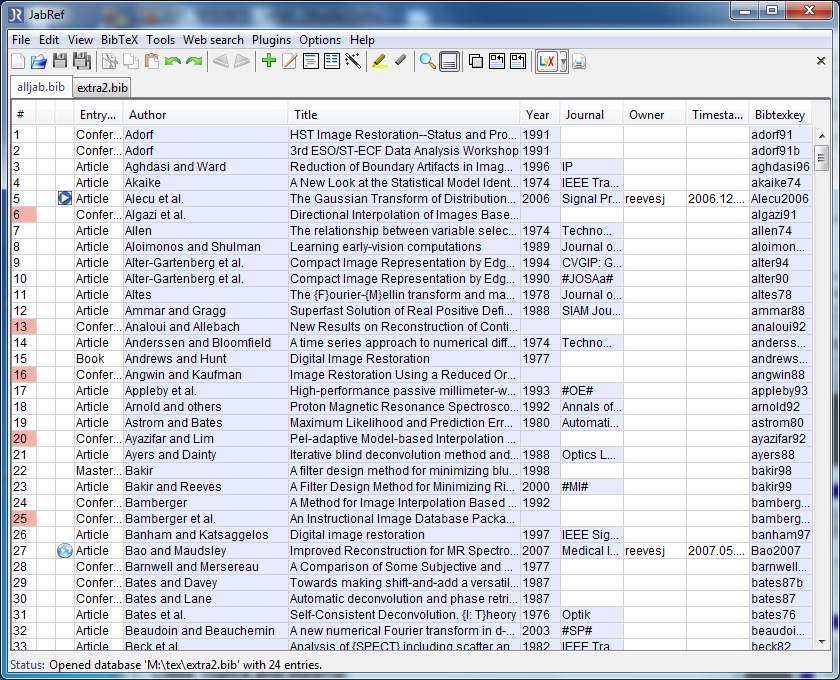
\includegraphics[width = 9.5cm]{jabref.png}
\end{figure}
}



\section{Prosper}
\frame { \frametitle{Presentations}

\setbeamercolor{uppercol}{fg=white,bg=ta3orange}%
\setbeamercolor{lowercol}{fg=black,bg=taorange}%
\begin{beamerboxesrounded}[upper=uppercol,lower=lowercol,shadow=true]
{\texttt{http://prosper.sourceforge.net/}}
\begin{itemize}
\item Prosper
\item Needs the following packages:
\begin{itemize}
\item prosper
\item seminar
\item pstricks
\end{itemize}
\end{itemize}
\end{beamerboxesrounded}

\begin{beamerboxesrounded}[upper=uppercol,lower=lowercol,shadow=true]
{\href{http://latex-beamer.sourceforge.net/}{http://latex-beamer.sourceforge.net/}}
\begin{itemize}
\item Beamer
\item Needs the following packages:
\begin{itemize}
\item latex-beamer
\item xcolor
\item pgm
\end{itemize}
\end{itemize}
\end{beamerboxesrounded}
}



\section{Beamer}
\begin{frame}[fragile]
\frametitle{Beamer documents}
\begin{itemize}
\item Uses the \texttt{frame} environment. A slide is defined within
\begin{verbatim}
%\begin{frame}
Slide body
%\end{frame}
\end{verbatim}
\item Preserves document structure
\item Very customizable
\item Allows for overlays
\pause
\item Auto-generation of ToCs and ToFs
\item Beamer tour:
\href{http://latex-beamer.sourceforge.net/beamerexample1.pdf}{http://latex-beamer.sourceforge.net/beamerexample1.pdf}.
\end{itemize}
\end{frame}




\section{Posters}
%%-----------------------------------------------------------------------


\frame {\frametitle{Posters}
\begin{itemize}
\item The a0poster.cls class file can be used to create upto A0 size posters.
\item It offers the following capabilities
\begin{itemize}
\item Allows for paper sizes A0, A1, A2, A3, \& A4
\item Allows font sizes from 12pt--107pt
\item Scales formulas and math symbols
\item The package also creates a postscript header file
for \texttt{dvips} to ensure that the poster will be printed in the right size.
\end{itemize}
\end{itemize}
}

%----------------------------------------------------------------------------
\begin{frame}[fragile]
\frametitle{a0poster.cls}
The header of a \LaTeX \ poster document looks like:
{\fontsize{8}{10}\selectfont
\begin{verbatim}
\documentclass[options]{a0poster}
\usepackage{graphicx,pstricks,...}
\begin{document}
\end{verbatim}}

The following options are available:

{\fontsize{8}{10}\selectfont
\begin{center}
\begin{tabular}{l|l}
{\slshape landscape} & landscape format\\
{\slshape portrait} & portrait format\\
{\slshape a0b} & ``DIN A0 big'' \\
{\slshape a0} & DIN A0\\
{\slshape a1} & DIN A1\\
{\slshape a2} & DIN A2\\
{\slshape a3} & DIN A3\\
{\slshape posterdraft} & reduces the postscript output to DIN A4 size.\\
{\slshape final} & makes postscript output in original size\\

\end{tabular}
\end{center}
}
\end{frame}


%%-----------------------------------------------------------------------


\frame {\frametitle{LyX}
\begin{itemize}
\item LyX is a \TeX\ based WYSIWYM editor
\item Available for multiple platforms
\item Offers a GUI with menus
\item Supports Bib\TeX\
\item Has WYSIWYG table and math editors
\item Uses \TeX\ rules for indents, spacing, and hyphenation
\end{itemize}
}

%%-----------------------------------------------------------------------


\frame {\frametitle{\LaTeX\ in plotting tools}
\begin{itemize}
\item MATLAB supports \LaTeX\
\begin{itemize}
\item Figure labels and other text can be parsed by a \LaTeX\ interpreter
\item The \texttt{latex} command translates MATLAB matrices into \LaTeX\ arrays
\item Can publish a formatted m-file, including \LaTeX\ constructs, as a \LaTeX\ document
\end{itemize}
\begin{figure}[!h]
\centering
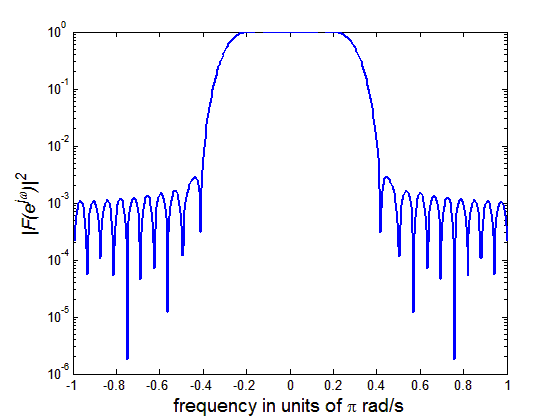
\includegraphics[width = 6.0cm]{matlab.png}
\end{figure}
\end{itemize}
}

\frame {\frametitle{\LaTeX\ in plotting tools}
\begin{itemize}
\item PGFPLOTS is a drawing package for \LaTeX based on PGF/Ti\textit{k}z
\item text-based specification of plots
\item can actually calculate and evaluate figures
\end{itemize}

}

%%--------------------------------------------------------------------------
\frame {\frametitle{\LaTeX \ at Auburn}
\begin{itemize}
\item Dr. E.E. Slaminka maintains AU theses style files
\item AU allows \LaTeX\ for theses.  Formatting restrictions have been relaxed.  Color and multimedia as well as hyper-references are possible in PDF files.
\item We have a rather inactive \texttt{tex-users} mailing list.
\end{itemize}
}


%%--------------------------------------------------------------------------
\frame {\frametitle{Summary}
\begin{itemize}
\item \LaTeX \ is a programming language, not an application
\item An abundance of \LaTeX \ utilities are available for different platforms
\item All \LaTeX \ components and packages are free and easily available
\item It can be used to generate various document types
\item Style files for Auburn University theses are available
\end{itemize}

}


\end{document}
